% Proposta de figura para a seção 2.2 (12/11/2026, pedido do autor). NÃO é
% parte do TG: o autor quer analisar antes de decidir. Figura em
% fig-periodos.tex (datas e procedência no cabeçalho dela), compilada pelo
% Makefile desta pasta.
\documentclass[11pt,a4paper]{article}
\usepackage[T1]{fontenc}
\usepackage[brazilian]{babel}
\usepackage{mathptmx}
\usepackage[a4paper,margin=2.4cm]{geometry}
\usepackage{graphicx}
\usepackage[font=small,labelfont=bf]{caption}
\usepackage[most]{tcolorbox}
\usepackage[hidelinks]{hyperref}
\setlength{\parskip}{0.45em}
\setlength{\parindent}{0pt}

\definecolor{cesc}{RGB}{220,50,32}
\definecolor{cmod}{RGB}{0,90,181}
\newtcolorbox{ideia}[1][]{colback=cmod!5, colframe=cmod!70, fonttitle=\bfseries, title={#1}, arc=2pt, boxrule=0.6pt}
\newtcolorbox{cuidado}[1][]{colback=cesc!4, colframe=cesc!70, fonttitle=\bfseries, title={#1}, arc=2pt, boxrule=0.6pt}

\title{Figura proposta para a seção 2.2\\[2pt]\large os períodos de teste, antes da otimização}
\author{Material de análise, fora do TG}
\date{12 de novembro de 2026}

\begin{document}
\maketitle

O TG fala dos períodos em dois lugares do Capítulo~II. O primeiro é a seção 2.2,
Caracterização do lugar e da amostra, que diz quais períodos foram estudados e por
quê. O segundo é a subseção Escolha da configuração, no plano experimental, onde a
Figura~7 mostra cada período de teste junto com os três anos de otimização que vêm
antes dele. Hoje só o segundo lugar tem figura. A proposta abaixo é uma versão
reduzida da Figura~7 para o primeiro lugar, só com os períodos de teste.

\section{A figura}

\begin{figure}[h]
\centering
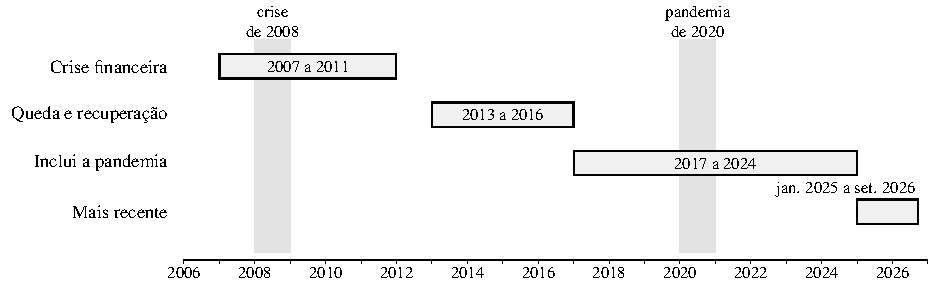
\includegraphics{fig-periodos.pdf}
\caption{Proposta para a seção 2.2 (título no TG: ``Períodos de teste'')}
\end{figure}

É a Figura~7 sem as barras escuras de otimização e sem a legenda, que deixa de ser
necessária quando só existe um tipo de barra. Cada linha é um período, com o rótulo
à esquerda dizendo o que o caracteriza, e as faixas cinza marcam 2008 e 2020, os
anos de crise que o Capítulo~III olha de perto. O eixo começa em 2006, e não em
2004 como na Figura~7, porque sem a otimização os três primeiros anos ficariam
vazios.

O leitor vê primeiro o que foi testado e, mais adiante, na Figura~7, como a
configuração de cada teste foi escolhida. As barras claras das duas figuras são as
mesmas, nas mesmas datas, de modo que a segunda parece a primeira com a otimização
acrescentada.

\begin{ideia}[De onde vêm as datas]
São as mesmas datas da Figura~7. As de 2007 a 2011, 2013 a 2016 e 2025 a 2026 vêm
da tabela do \texttt{dados/resultados/refeito\_2026-10-05/PROTOCOLO.md}. As de 2017
a 2024 vêm da primeira e da última linha da \texttt{curva\_R6\_GS.csv} (02/01/2017
e 27/12/2024). A posição de cada barra é calculada a partir da data, no próprio
desenho.
\end{ideia}

\section{Onde entraria}

No fim da seção 2.2, logo depois do parágrafo que começa com ``O recorte temporal
foi dividido em períodos''. A norma exige que toda figura seja chamada no texto, e
basta uma frase no fim desse parágrafo, por exemplo: ``A Figura~X mostra esses
períodos.'' O título sugerido é ``Períodos de teste'', com ``Fonte: Elaboração
própria.'' embaixo.

Como ela vem antes da Figura~7 no texto, a numeração das figuras seguintes sobe uma
unidade: a atual Figura~7 passa a ser a 8, e assim por diante. No LaTeX isso é
automático, já que as chamadas usam \verb|\ref|.

\section{Pontos para decidir}

\begin{cuidado}[Os rótulos das linhas]
Na proposta, os rótulos seguem as palavras da seção 2.2: crise financeira, queda e
recuperação, inclui a pandemia e mais recente. A Figura~7 usa ``Crise de 2008'' e
``Teste principal'' na primeira e na terceira linha. O nome ``teste
principal'' só é explicado no Capítulo~III, e por isso não foi usado na seção 2.2.
Ficam três caminhos. O primeiro é deixar como está, com cada figura usando as
palavras do trecho em que aparece. O segundo é trocar os rótulos da Figura~7 pelos
desta. O terceiro é usar os da Figura~7 também aqui. O segundo deixa as duas
figuras iguais nas partes comuns, que é o mais fácil de acompanhar.
\end{cuidado}

\begin{cuidado}[Repetição]
As duas figuras mostram as mesmas barras claras. A repetição é intencional, porque
cada uma responde a uma pergunta diferente (o que foi testado e como foi escolhido),
mas a banca pode estranhar duas linhas do tempo parecidas no mesmo capítulo. A frase
que chama a Figura~7 pode lembrar a relação, por exemplo: ``A Figura~X acrescenta à
Figura~Y os períodos de otimização.''
\end{cuidado}

As outras três ações foram testadas nos mesmos quatro períodos (o teste
complementar, 2.5.8). A figura não as menciona, porque a seção 2.2 apresenta as
ações no parágrafo anterior.

\end{document}
